% !TeX program = xelatex
% !TeX encoding = UTF-8
\documentclass{MathorCupModeling}
\usepackage{mwe,color,float}
\usepackage[linesnumbered,ruled]{algorithm2e}
\everymath{\displaystyle}

\extrafloats{100}
\bianhao{MC2305806}
\tihao{D}
\timu{\textbf{题目}}
\keyword{关键词两个之间分号隔开}
\begin{document}
	\begin{abstract}
		这里是摘要部分
	\end{abstract}

	\pagestyle{empty}
	\tableofcontents
	\newpage
	\pagestyle{fancy}

	\setcounter{page}{1}
	\section{问题的提出}
	\subsection{问题背景}
	改革开放以来,我国民航业蓬勃发展,越来越多的乘客选择乘坐飞机出行,飞行安全的重要性不言而喻。截至2022年3月21日,即“3.21”空难发生前,我国民航安全飞行达1亿零59万飞行小时,为我国历史最好安全记录。严重的飞行安全事故不仅会使航空公司蒙受经济损失,还威胁着乘客的生命财产安全。为科学管理,降低飞行事故发生的几率,综合现有数据进行监测并预警风险,总结出具有针对性和系统性的方案提升从业人员素质显得尤为重要。在航空安全数据分析中快速存取记录器(Quick Access Recoder,QAR)发挥着重要作用。目前我国民航业主要研究两方面:
	\begin{itemize}
		\item 超限事件的研究,分析及应用;
		\item 非超限数据的统计分析及应用。
	\end{itemize}其中,对于前者的分析着眼于超出阈值的部分,然而超出阈值的部分不完全是人为因素,可能为环境或飞机本身存在一定问题,若基于非人为因素对机组严以要求显然是不合理的。QAR超限可为航空安全管理和飞行训练提供数据支撑,而少量的QAR超限显然不具有说服性,故挖掘QAR全航段数据,基于不同飞行机组,航线,机场及特殊飞行条件下的飞行记录,建立数学模型,并分析之,评估各指标风险系数,针对性开展安全培训,排除安全隐患,改进安全绩效。
	\subsection{问题要求}
	\begin{itemize}
		\item \textbf{问题一}:由于QAR数据并不能保证绝对正确性,故应进行数据预处理减少错误数据干扰。在此基础上对附件1进行可靠性研究,提取关键数据项并分析重要程度。
		\item \textbf{问题二}:飞行过程往往通过一系列飞行操纵如:横滚、俯仰等以保证安全。国内航司主要以超限监控飞行动态,虽然能够快速分辨飞机状态偏差,但无法在较短时间内知道原因。为解决此问题,请依据附件1合理量化描述飞行操纵。
		\item \textbf{问题三}:除人为,环境,飞机本身缺陷外等因素外,仍有一定因素会影响超限的发生。请依据附件2分情况讨论超限并研究其基本特征。
		\item \textbf{问题四}:飞机运行数据研究往往由两大类组成,一类由LOSA获取,另一类则遵从相关学者建议,开展飞行技术评估。请依据附件3,建立数学模型以合理分析评估飞行员飞行技术。
		\item \textbf{问题五}:在QAR实现陆空实时传输的情况下,以航司安全管理人员的身份建立实时自动化预警机制,预防可能的安全事故,并依据附件1给出仿真结果。
	\end{itemize}

	\section{问题的分析}
	\subsection{问题的整体分析}
	该问题是一个关于航空安全风险及飞行技术的数据分析、建立预警模型的问题。
	
	\textbf{从分析目的看},本题需要分析飞机在飞行中的各项飞行参数和航空安全风险,同时建立自动化预警机制,从而预防安全事故的发生。因此本主题需要完成两方面任务:其一,研究飞行参数对航空安全的影响程度,并对各参数进行量化分析。其二,根据上述分析,建立合理模型,通过飞行参数对风险进行识别,改进安全绩效。确保模型的准确性、稳健性、可靠性,并有一定的泛化能力。

	\textbf{从数据来源、特征看},本题的数据来源于某航司2013-2017年随机快速存取记录器(QAR)。数据包括2014年7月5日至2014年10月11日部分时段某些航线完整飞行数据;2015年至2016年间相关航线超限数据;2013年至2017年间A机型落地主操作人员资质及相关飞行数据。飞行及超限数据量较大且影响飞行及超限数据的因素具有存在无效值、高维、复杂等特征。因此本题数据较为特殊且复杂,需对数据进行预处理,便于后续问题的分析。
	
	\textbf{从模型的选择看},

	\textbf{从编程软件的选择看},本题为大数据分析类,需要进行大量的数据预处理、数据分析、数据可视化,并依据各设问建立预警自动化只能预警机制,因此我们选择Python Jupyter对问题进行求解,其交互式的编程范式及轻量化,方便且高效。
	
	\subsection{问题一的分析}
	问题一的核心目的有以下几点:{\heiti 其一},\textbf{对真实的QAR数据进行预处理,去伪存真};{\heiti 其二},\textbf{分析研究附件一数据质量的可靠性};{\heiti 其三},\textbf{提取一项飞行安全的关键性因素,并定性及定量分析}。对于已给的数据集,数据在真实性、完整度、指标标准等方面存在一定缺陷,这导致我们在原始数据上不可直接进行分析,因此需要对其进行相应的预处理。此外附件1为8次航班的由起飞到降落的全过程的QAR数据,数据体量大,因此我们需要由特殊到一般,建立普适性模型,高效分析多张数据表格;同时我们还发现,数据维度较高,为得到关键性因此,考虑累计方差解释、层次聚类分析及熵权法,确定重要度较高指标,并对筛选出的指标进行合理性分析。
	\subsection{问题二的分析}
	问题二的核心目的在于\textbf{对着陆时的飞行操纵进行量化描述}。由于在飞行过程中,航空公司只能监测到飞机飞行时的操纵动作,虽然能分辨出是否否出现偏差,确无法得出原因,因此我们需要对操纵进行量化描述。通过预处理后附件一的数据,我们绘制出了八个航线飞机的状态和操纵随时间变化的曲线图,通过曲线的突变,来合理分析发生偏差的原因。
	\subsection{问题三的分析}
	问题三的核心目的有以下几点:{\heiti 其一},\textbf{基于附件2中的数据对所有超限情形进行筛选,分类处理};{\heiti 其二},\textbf{分析超限事件发生的各种情形};{\heiti 其三},\textbf{总结研究得出不同超限的基本特征}。对于所给定的数据集,数据多且杂乱无章,我们无法直接分析,故我们对附件2中的数据进行了筛选,剔除了空白和未知部分的无效数据,而后对各超限情形进行了分类,共分为6类。考虑到数据集提供了日期,起飞机场,目的机场等数据,故我们从季节,航线,机场等角度进行了统计,为便于分析,我们将相关情形做出可视化处理并建立模型,而后对其进行研究以得出不同超限的基本特征。
	\subsection{问题四的分析}
	问题四的核心目的在于\textbf{基于飞行参数对飞行员的技术进行评估}。但是附件3与附件1同样在数据完整度、指标标准等方面存在一定缺陷,因此我们也需要对其进行一定的预处理;同时,我们还发现附件3维度更高,飞行参数较多,对于模型的效率有一定影响,因此我们沿用问题一的想法,以累计方差解释确定重要因素较高的指标的个数,再以随机森林及极端梯度提升算法综合分析出与飞行员飞行技术重要程度较高的因素。但我们还发现,附件3中,飞行员资质为“C”类的占比仅为整体的$0.844\,\%$,因此我们综合多方面考虑,选择将该两项数据单独分析,剩余数据视为多分类预测。最后以筛选出的重要指标为自变量,飞行员的“不同资质”,即不同技术级(除“C”类)别为因变量,建立XGboost多分类预测模型,从而建立出基于飞行参数的飞行技术评估方法。同时,为探讨模型效果,我们绘制出模型的{\heiti 分类混淆矩阵热力图}、{\heiti 分类报告}、{\heiti ROC/AUC	曲线}等对预测结果进行合理性分析。
	\subsection{问题五的分析}

	\section{模型的假设}
	\begin{itemize}
		\item \textbf{假设一}:
		\item \textbf{假设二}:
		\item \textbf{假设三}:
		\item \textbf{假设四}:
	\end{itemize}
	\section{符号说明},
	\begin{center}
		\begin{tabularx}{0.7\textwidth}{c@{\hspace{1pc}}|@{\hspace{2pc}}X}
			\Xhline{0.08em}
			符号 & \multicolumn{1}{c}{符号说明}\\
			\Xhline{0.05em}
			$\mu$ & 样本平均数 \\
			$\alpha$ & 系数 \\
			$\beta$ & \\
			$\omega$ & \\
			$\sigma$ & 标准差 \\
			\Xhline{0.08em}
		\end{tabularx}
	\end{center}

	\section{模型的建立与求解}
	对于本题,本文模型的建立与求解部分主要分为数据的准备,模型的建立、求解、结果分析。
	\begin{itemize}
		\item \textbf{数据的准备}:对于给定的数据集进行预处理,方便后续模型的建立,以及多次航班的规范分析。
		\item \textbf{模型的建立、求解、结果分析}:对于给定的数据集,本文依据其特点,建立合适的模型,研究并量化分析影响飞行安全的因素。此外还需要分析飞行阶段操纵杆的过程变化情况,分析安全性。同时,还需要依据飞行参数对驾驶员飞行技术进行预测,并解释预测的合理性。最后需要结合上述问题,建立自动化智能预警机制,预防可能的安全事故的发生,给出仿真结果。
	\end{itemize}
	\subsection{问题一模型的建立与求解}
	对于问题一,我们首先分析数据的特点,依据时间特征及对应的各参量进行合理性分析,对错误值进行剔除,提高数据的真实性,并以此分析数据的可靠性;之后我们依据刘柳\textcolor{blue}{\cite{Paper:刘柳}}、龙海江\textcolor{blue}{\cite{Paper:龙海江}}学者的研究结成果,采用层次聚类法对多维度指标进行聚类分析,同时在此基础上利用主成分分析累计方差解释,确定影响飞行安全的关键性指标,并利用熵权法对其重要性进行量化分析。此外注重定性及定量的分析研究,结果与现实情况相近,选取结果良好。
	\subsubsection{附件1数据预处理}
	通过对附件1的8个Excel表格依此分析,并结合快速存取记录器(Quick Access Recoder,QAR)数据的特点,我们发现以下几点可能的错误方面:
	\begin{itemize}
		\item \textbf{起始时刻不为飞机开始运行时刻}:通过对8张表8次航班的全航段记录数据的逐一分析,我们发现表格“201404091701”记录器开始记录的时刻为2014年4月9日14时23分51秒,而该航班实际运行时间应该为2014年4月9日17时01分50秒,因此我们认为该表格的起始时刻不应为前者,而应是飞机开始运行的时刻。因此我们将该表格的起始时刻校正,即删除14时23分51秒的数据,保留17时01分50秒之后的数据。而对于其余表格并未发现相同错误。
		\item \textbf{相邻数据存在时刻上的重复且后续指标不一致}:利用Python的pandas库,对8张表格统一分析,发现所有表格均存在该方面的问题,即存在某同一时刻的数据,但后续指标却不一致,如\textcolor{blue}{\cref{tab:时刻重复值}}所示,这是明显的QAR数据记录错误,究其原因,可能是由于该时刻被QAR连续记录两次,但指标发生变化,但为了保证数据的在时刻上的连续性,我们以这些重复时刻数据首次出现的为标准,将其保留,而另一条数据选择剔除。
\begin{table}[htbp]
	\centering
	\caption{表格“201404101159”时刻重复值(部分列)}
	\scalebox{0.85}{
	  \begin{tabular}{cccccccc}
	  \toprule
	  \textbf{月} & \textbf{日} & \textbf{具体时间} & \textbf{海拔高度} & \textbf{下降率} & \textbf{无线电高度} & \textbf{计算空速} & \textbf{地速} \\
	  \midrule
	  4     & 10    & 12:18:16 & 12751 & -3144 & 1404  & 310.625 & 372.25 \\
	  4     & 10    & 12:18:16 & 12804 & -3154 & 1404  & 310.75 & 372.5 \\
	  4     & 10    & 13:11:44 & 30103 & 2     & 1404  & 305.625 & 465.25 \\
	  4     & 10    & 13:11:44 & 30105 & -10   & 1404  & 305.625 & 465.25 \\
	  \bottomrule
	  \end{tabular}}
	\label{tab:时刻重复值}
\end{table}

		\item \textbf{出现两列一致指标,且其下所有时刻数据一致}:我们发现附件1的8次航班数据中均出现两次“俯仰角率”列数据,为了探讨其下所有时刻数据是否一致,我们利用pandas对其进行分析,发现该两列数据无任何差别,造成数据冗余,因此我们将其中一列剔除。
	\end{itemize}

	经过上述处理后,各表格行数据剔除率及数据保留率如\textcolor{blue}{\cref{tab:数据剔除率及保留率}}所示。各表格列数据均剔除一列。
\begin{table}[H]
	\centering
	\caption{附件1各表格数据剔除、保留率(名称省略年份2014)}
	\scalebox{0.85}{
	  \begin{tabular}{ccccccccc}
	  \toprule
	  \textbf{Rate} & \textbf{070532} & \textbf{071917} & \textbf{080617} & \textbf{081034} & \textbf{090110} & \textbf{091701} & \textbf{100843} & \textbf{101159} \\
	  \midrule
	  剔除率   & 0.000284  & 0.000299  & 0.000301  & 0.000286  & 0.000315  & 0.000357  & 0.000429  & 0.000268  \\
	  保留率   & 0.999716  & 0.999701  & 0.999699  & 0.999714  & 0.999685  & 0.999643  & 0.999571  & 0.999732  \\
	  \bottomrule
	  \end{tabular}}
	\label{tab:数据剔除率及保留率}
\end{table}
	为了再次验证数据在时刻层面的连续性,即每行记录的数据均间隔为1秒,我们对所有航班进行时刻点计算,均与处理后的数据记录条数一致,从而也反映出保留下的数据的合理性。但此处,我们并未对其他方面进行分析,如异常值等,也并未对其进行剔除,这是由于我们查阅相关资料,结合李瀚明\textcolor{blue}{\cite{Paper:李瀚明}}学者及胡占桥老师\textcolor{blue}{\cite{Paper:胡占桥}}的研究,及对实际数据的分析,给出下几点原因:\begin{itemize}
		\item \textbf{传感器存在一定误差},QAR误差可分为三种:多报、漏报、误报。多报即为生成了额外的数据点,造成数据冗余;漏报即为未生成相应时刻的数据点;误报即为某些点因QAR仪器,造成数据采集有误;
		\item \textbf{QAR存在一定局限性},记录的数据可能会有少部分产生问题,但浮值不会变化过大,这是由仪器本身所决定,而时刻数据(上述分析的多报)即为其局限性的一方面;
		\item \textbf{部分异常值可能为机组人员误操作造成},即我们很难在一定程度上区分误报与机组人员误操作造成异常值记录的数据,若我们将其剔除,则会使原始数据在信息解释方面造成一定失真,对数据进行了“篡改”,从而影响后续分析。
	\end{itemize}
	因此在这里,我们不考虑部分异常值,而尽可能保留数据的真实性,而对于该数据,我们也将在问题五进行详细叙述。

	同时我们发现,附件1的8张表格,前三行均属于表头类型,且有部分字段重复,若将其直接利用pandas读取,可能会对后续处理产生一定影响,因此我们根据附件1的字段中文说明,将8张全航段表格数据表头进行处理,且保证所有表格表头一致,方便后续处理。

	此外,通过读取附件1数据,查看其空缺值情况,发现“起落架”\textcolor{blue}{\footnote{这里指标名称已由原数据的英文修改为中文指标。}}该列数据缺失值较多,这里我们以附件1中表格“201404101159”为例\textcolor{blue}{\footnote{对于问题一,在本文正文,我们均以附件1中表格“201404101159”为例进行分析,后文简称”航线8“,其余表格的分析结果也将在正文及附录中呈现。}},其空缺值情况如\textcolor{blue}{\cref{fig:附件1航班8缺失值}}所示。
	\begin{figure}[H]
		\centering
		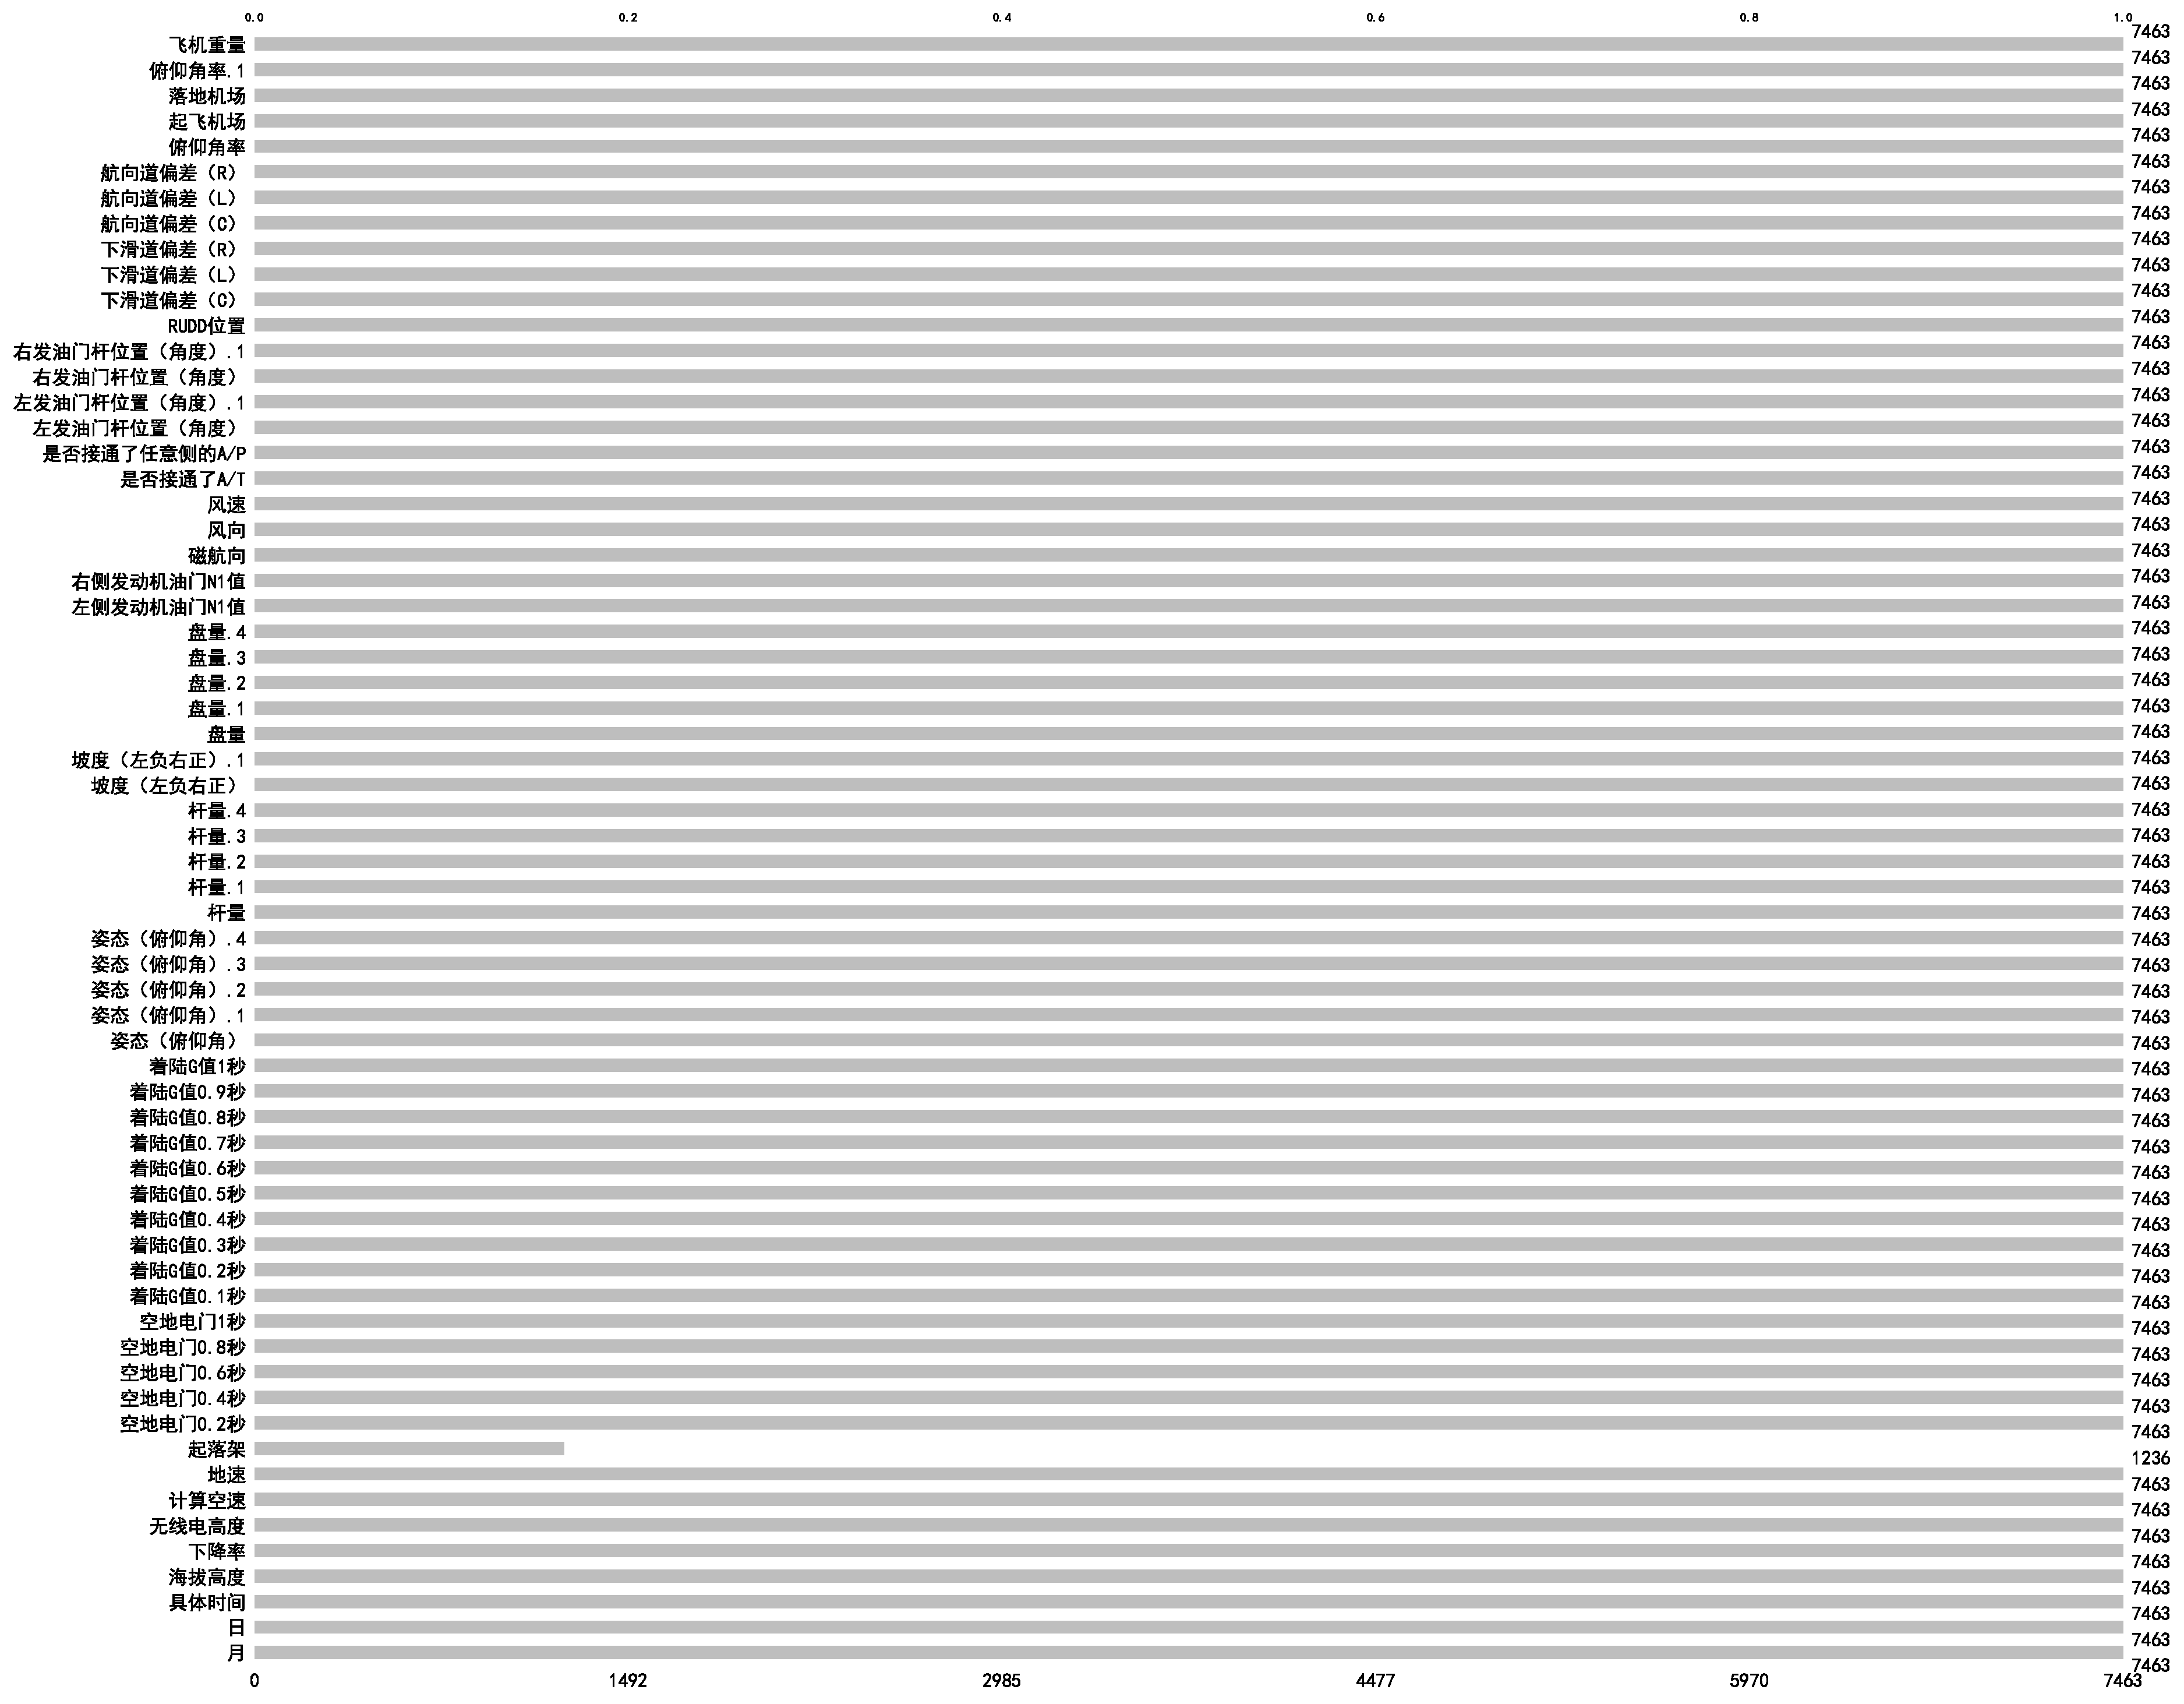
\includegraphics[width=0.66\linewidth]{附件1航班8缺失值.pdf}
		\caption{附件1航班8缺失值}
		\label{fig:附件1航班8缺失值}
	\end{figure}
	
	这里,我们结合实际分析,认为空缺值均应填充为“NON-DOWN”,即此时起落架为收起状态,理由如下:
	\begin{itemize}
		\item “起落架”该列数据存在的均为“DOWN”,即起落架状态为放下状态,结合具体时刻,我们可以发现为飞机运行的开始阶段与将要结束阶段,因此中间的缺失值视为在空中正常飞行阶段;
		\item 结合“海拔”、“空地电门”等多项列数据进行分析,可以验证上述我们的猜想,即中间段“起落架”的缺失值均为“NON-DOWN”。
	\end{itemize}

	因此在这里我们首先以该值进行填充,而其余处理也将在后续展开叙述。此外,我们发现除该列数据缺失,其余列数据均无一缺失,则无需再进行填充处理。

	同时,我们还注意到数据表中“起落架”“空地电门”“是否接通了A/T”“是否接通了任意侧的A/P”“起飞机场”“落地机场”指标的数据均为文本类型数据,对于后续的分析及模型的建立有一定影响,因此我们这里采用字典方法,对其键值对人为对应替换,替换结果如\textcolor{blue}{\cref{tab:附件1指标替换}}所示。其中“起飞机场”与“落地机场”列数据,我们选择直接剔除,而将在后续与“月”“日”一起进行定性分析。
\begin{table}[H]
	\centering
	\caption{附件1指标替换}
	\scalebox{0.85}{
	  \begin{tabular}{cc}
	  \toprule
	  \textbf{指标} & \textbf{替换} \\
	  \midrule
	  起落架   & DOWN:1,NON-DOWN:0 \\
	  空地电门  & True:1,False:0 \\
	  是否接通了A/T & DISENGD:0,ENGAGED:1 \\
	  是否接通了任意侧的A/P & OFF:0,ON:1 \\
	  \bottomrule
	  \end{tabular}}
	\label{tab:附件1指标替换}
\end{table}

	最后,我们发现附件1的维度较高,且各维度数据量纲不一,对后续模型的建立会产生较大影响,因此这里我们对所有数据进行标准化及归一化处理,其区别、后续利用方式及计算方式如下:
	\begin{itemize}
		\item \textbf{数据标准化}:采用\textbf{Z-score}方法处理,用于主成分分析(Principal Component Analysis,PCA)累计方差贡献率(Cumulative Variance Contribution Rate,CVCR)及层次聚类(Hierarchical Clustering,HC)模型的建立。同时该标准化处理方法适合当代嘈杂的大数据场景\textcolor{blue}{\cite{Paper:标准化}}。因此对于大样本的数据,如出现部分异常值,使用该方法对最终结果影响较小。其计算方式如下:
		
		对于某一列数据$x=\left[x_1,x_2,\cdots,x_m\right]^{\mathrm{T}}$,其平均值为
		\begin{equation}
			\mu=\frac{1}{m}\sum_{i=1}^{m}x_i \label{fmean}
		\end{equation}
		标准差为
		\begin{equation}
			\sigma=\sqrt{\frac{1}{m}\sum_{i=1}^{m}\left(x_i-\mu\right)^2} \label{fstd}
		\end{equation}
		则标准化后的数据为
		\begin{equation}
			\left(x_{\mathrm{Z-score}}\right)_i=\frac{x_i-\mu}{\sigma} \label{Z-score}
		\end{equation}
		\item \textbf{数据归一化}:采用\textbf{Min-Max}方法处理,用于熵权法(Entropy Weight Method,EWM)模型的建立。其处理方法计算公式如下\textcolor{blue}{\footnote{此处仅为理论公式,而在EWM模型建立中将进行更深层次叙述。}}:
		\begin{equation}
			\left(x_{\mathrm{Min-Max}}\right)_i=\frac{x_i-\mathrm{min}\left(x\right)}{\mathrm{max}\left(x\right)-\mathrm{min}\left(x\right)} \label{Min-Max}
		\end{equation}
	\end{itemize}
	这样分开分别处理有以下几点原因:
	\begin{itemize}
		\item \textbf{Z-score}方法,使得原数据经过处理后,数据集中于0附近,即均值为0,标准差为1。其适用于PCA-CVCR及HC模型的建立,大大提升模型的效率。
		\item \textbf{Min-Max}方法,使得原数据经过处理后,在设定的最大值与最小值之间,方便EWM的建立,避免对数运算的错误。
	\end{itemize}
	\subsubsection{模型的建立}
	对于问题一,我们建立PCA-CVCR、HC及EWM模型,过程如下分析。

	\textbf{主成分分析累计方差贡献率(Principal Component Analysis Cumulative - Variance Contribution Rate,PCA-CVCR)}:由于附件1所有数据集较为复杂,且为高维数据,而PCA作为一种可以将原始高维数据转换为新的低维数据的方法,故我们采用此方法对数据集进行处理。在此我们将对PCA累计方差解释率作出解释。在PCA过程中,各主要成分所占方差比例的累加和,往往以百分比的方式呈现。PCA累计方差解释率对选择合适的主成分进行降维起到至关重要的作用。在PCA降维中我们往往基于PCA累计方差解释率的高低来选择一定数量的主成分以代表原始数据的特征,PCA累计方差解释率越高,说明前几个主成分所能代表的方差比例越高,便可选择这些主成分降维以保留更多信息。其计算方式如下:
	
	根据标准化后的数据集计算协方差矩阵
	\begin{equation}
		\boldsymbol{C}=\left[ \begin{matrix}
			\text{Cov}\left( X_1,X_2 \right)&		\text{Cov}\left( X_1,X_2 \right)&		\cdots&		\text{Cov}\left( X_1,X_n \right)\\
			\text{Cov}\left( X_2,X_1 \right)&		\text{Cov}\left( X_2,X_2 \right)&		\cdots&		\text{Cov}\left( X_2,X_n \right)\\
			\vdots&		\vdots&		\ddots&		\vdots\\
			\text{Cov}\left( X_n,X_1 \right)&		\text{Cov}\left( X_n,X_2 \right)&		\cdots&		\text{Cov}\left( X_n,X_n \right)\\
		\end{matrix} \right] \label{C}
	\end{equation}
	其中,每一个元素定义如下\textcolor{blue}{\cite{Paper:概率论与数理统计}}
	\begin{equation}
		\text{Cov}=\left( X,Y \right)=E\left\{\left[X-E\left(X\right)\right]\left[Y-E\left(X\right)\right]\right\}=E\left(XY\right)-E\left(X\right)E\left(Y\right) \label{Cov}
	\end{equation}
	其中$E\left(X\right)$为该列数据的均值。

	之后,计算上述协方差矩阵的特征值$\lambda_n$及其对应的特征向量$\boldsymbol{u}_{nj}$,这里我们不妨令$\lambda_1\geqslant\lambda_2\geqslant\cdots\lambda_n\geqslant 0$,由特征向量组成$n$和新的指标变量
	\begin{equation}
		\left\{ \begin{array}{l}
			y_1=\boldsymbol{u}_{11}x_1+\boldsymbol{u}_{21}x_2+\cdots +\boldsymbol{u}_{n1}x_n\\
			y_2=\boldsymbol{u}_{12}x_1+\boldsymbol{u}_{22}x_2+\cdots +\boldsymbol{u}_{n2}x_n\\
			\vdots\\
			y_3=\boldsymbol{u}_{1n}x_1+\boldsymbol{u}_{2n}x_2+\cdots +\boldsymbol{u}_{nn}x_n\\
		\end{array} \right. 
	\end{equation}
	其中$y_n$是第$n$个主成分,再计算个主成分的贡献率$\gamma_n$及累计贡献率$\alpha_p$
	\begin{equation}
		\gamma_n=\frac{\lambda_n}{\sum\limits_{i=1}^n\lambda_i}
	\end{equation}
	\begin{equation}
		\alpha_p=\frac{\sum\limits_{i=1}^p\lambda_i}{\sum\limits_{i=1}^{n}\lambda_i}\left(p\leqslant n\right)
	\end{equation}
	
	通过上述步骤,我们绘制出航线8各指标参量的累计方差解释图,如\textcolor{blue}{\cref{fig:附件1-8累计方差解释}}所示。
	\begin{figure}[H]
		\centering
		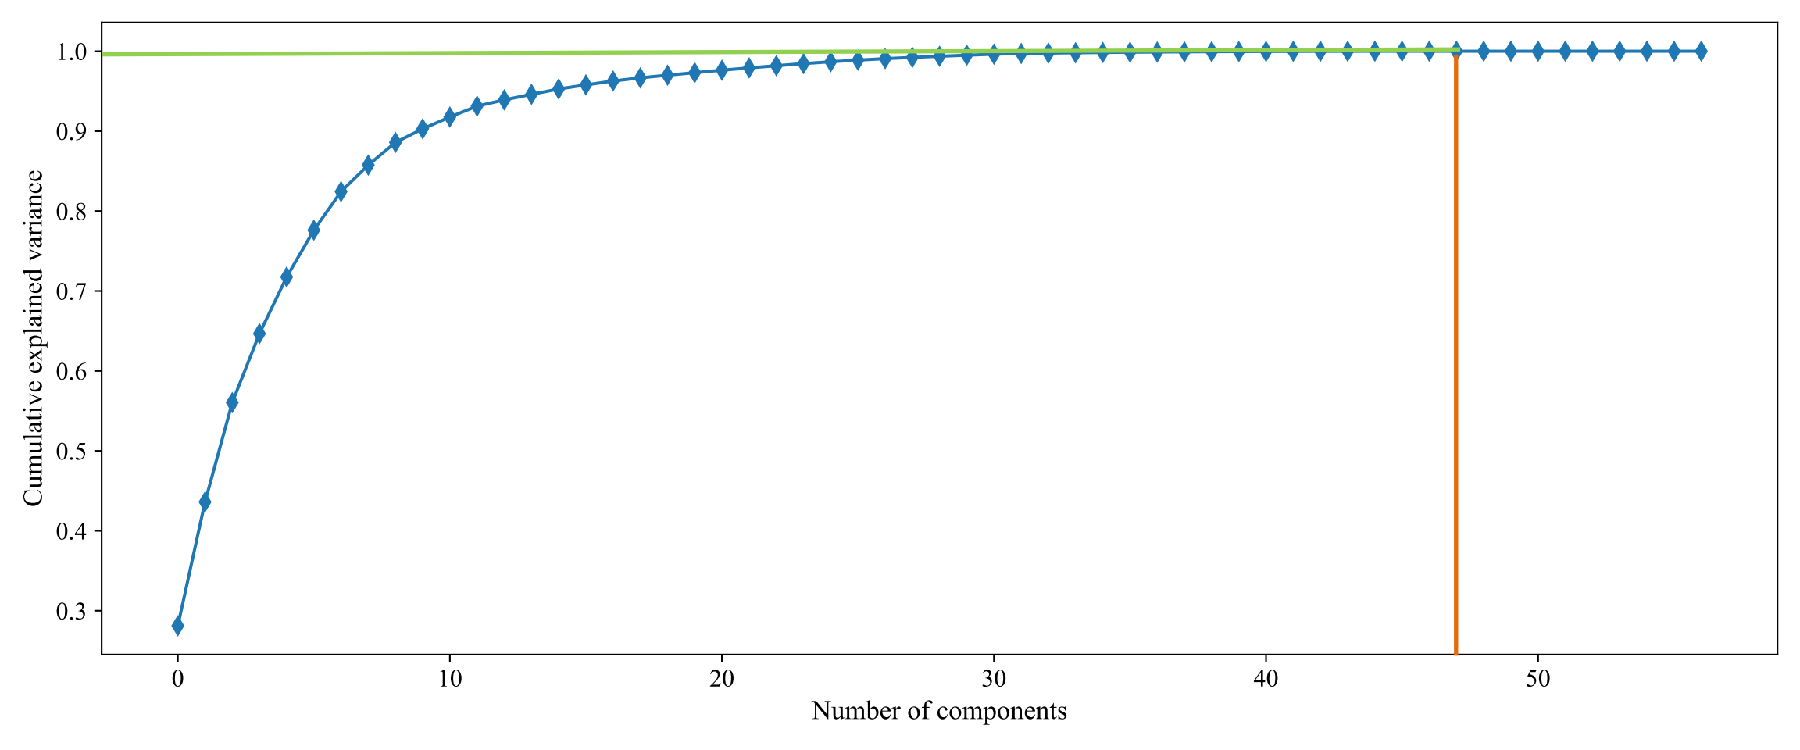
\includegraphics[width=0.85\textwidth]{1-8 PCA Cumulative explained variance.pdf}
		\caption{航线8各指标参量的累计方差解释}
		\label{fig:附件1-8累计方差解释}
	\end{figure}

	依据上图,我们可以发现在指标个数为47个左右时,指标对于信息的累计方差贡献率趋近于$100\,\%$,因此,初步分析后,我们将在后续选择近似47个指标进行综合分析。

	\textbf{层次聚类(Hierarchical Clustering,HC)}是基于簇间的相似度在不同层次上分析数据,从而形成树形的聚类结构,采用自底向上策略。首先将每个对象作为单独的一个原子簇,然后合并这些原子簇形成越来越大的簇,直到所有的对象都在层次的最上层。\textcolor{blue}{\cite{Paper:层次聚类}}我们定义类与类间相似度度量:若有两个样本$G_1$与$G_2$,则可用“ward”方法,即离差平方和法度量他们之间距离:
	\begin{equation}
		D_1=\sum_{x_i\in G_1}{\left( x_i-\overline{x_1} \right)}^{\text{T}}\left( x_i-\overline{x_1} \right) 
	\end{equation}
	\begin{equation}
		D_2=\sum_{x_j\in G_2}{\left( x_j-\overline{x_2} \right)}^{\text{T}}\left( x_j-\overline{x_2} \right)
	\end{equation}
	\begin{equation}
		D_{12}=\sum_{x_i\in G_1\cup G_2}{\left( x_k-\overline{x} \right)}^{\text{T}}\left( x_k-\overline{x} \right)
	\end{equation}
	其中
	\begin{equation}
		\overline{x_1}=\frac{1}{n_1}\sum_{x_i\in G_1}x_i
	\end{equation}
	\begin{equation}
		\overline{x_2}=\frac{1}{n_2}\sum_{x_j\in G_2}x_j
	\end{equation}
	\begin{equation}
		\overline{x}=\frac{1}{n_1+n_2}\sum_{x_k\in G_1\cup G_2}x_k
	\end{equation}
	因此,可以得到
	\begin{equation}
		D\left(G_1,G_2\right)=D_{12}-D_1-D_2
	\end{equation}

	根据上述计算方法,我们绘制出层次聚类树状图,如\textcolor{blue}{\cref{fig:1-8层次聚类}}所示。\textcolor{blue}{\footnote{由于数据维度过高且字段过长,我们将其列为阿拉伯数字,而最后结果也将在后文提及。}}
	\begin{figure}[H]
		\centering
		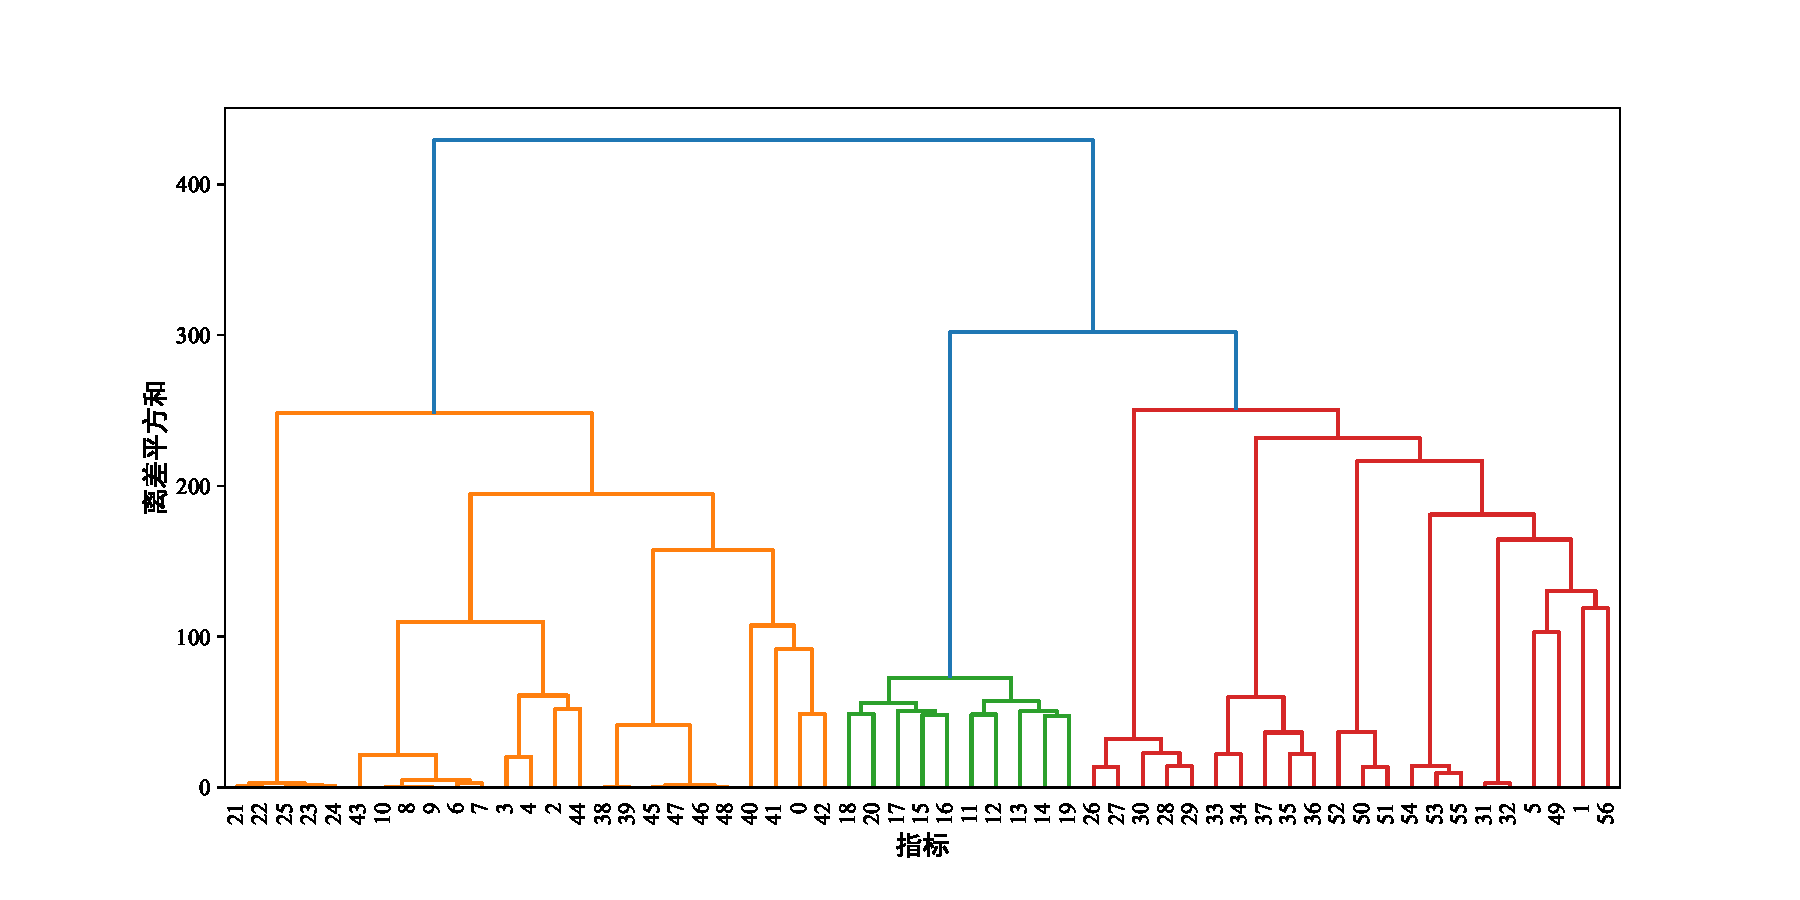
\includegraphics[width=0.85\textwidth]{1-8 层次聚类树状图.pdf}
		\caption{各指标参量的层次聚类树状图}
		\label{fig:1-8层次聚类}
	\end{figure}

	根据以上结果,并结合附件1的其余7次航班分析结果,我们最终确定“人-机-环”评级体系,即三方面:人为操作、机器状态、环境干预。并依据社会实际情况,确定了最终三个层面的共计47个指标,但实际上,一部分指标是一种指标不同时刻的量值。因此,在这里我们将其进行合理性合并,最终得到三个层面共计19项与飞机飞行安全高度相关的指标,即:
	\begin{itemize}
		\item \textbf{环境干预}:风向、风速;
		\item \textbf{人为操作}:下降率、地速、起落架、着陆G值、杆量、盘量、RUDD位置;
		\item \textbf{飞机状态}:姿态(俯仰角)、航向道偏差、磁航向、左侧发动机油门N1值、右侧发动机油门N1值、下滑道偏差、左发油门杆位置(角度)、右发油门杆位置(角度)、坡度(左负右正)、俯仰角率。
	\end{itemize}

	下面我们将对上述重要程度较高的因素进行量化分析,这里我们使用熵权法进行分析。此外我们还需要对前文叙述的部分因素进行定性分析。

	\textbf{熵权法(Entropy Weight Method, EWM)}是一种指标客观影响程度的量化方法。当信息熵越大时,信息的无序程度越大,此时,信息价值越小,指标权重就越小\textcolor{blue}{\cite{Paper:EWMO}}。其计算步骤如下:
	\begin{itemize}
		\item \textbf{Step 1}:指标正向化。由于数据集构成的指标类别不一,部分指标可能数值越大越好,部分指标可能越小越好,而有的可能在某一点取值最优,为方便、高效评价,我们需要进行指标正向化处理\textcolor{blue}{\cite{Paper:EWMT}}。其处理方法如下
		\begin{itemize}
			\item {\heiti 越大越优指标}
			\begin{equation}
				x'_{ij}=x_{ij} \label{fmax}
			\end{equation}
			\item {\heiti 越小越优指标}
			\begin{equation}
				x'_{ij}=\mathrm{max}\left(x_{ij}\right)-x_{ij} \label{fmin}
			\end{equation}
			\item {\heiti 在$\beta$处取值最优指标}
			\begin{equation}
				x'_{ij}=1-\frac{\left|x_{ij}-\beta\right|}{\mathrm{max}\left(\left|x_{ij}-\beta\right|\right)} \label{fmid}
			\end{equation}
		\end{itemize}
		\item \textbf{Step 2}:数据标准化。由于数据集构成的指标数据数量级存在差异、量纲不一,为消除上述情况对结果的影响,我们需要将各指标进行标准化处理,这里我们使用Min-Max方法。处理方法计算公式为
		\begin{equation}
			r_{ij}=\frac{x'_{ij}-\mathrm{min}\left(x'_{j}\right)}{\mathrm{max}\left(x'_{j}\right)-\mathrm{min}\left(x'_{j}\right)} \label{Min-Max}
		\end{equation}
		\item \textbf{Step 3}:计算信息熵。进行上述处理后可得到由特征数据构成的矩阵$R\left(r_{ij}\right)_{m\times n}$,对于某一项指标的数据$r_j$,其信息熵为
		\begin{equation}
			E_j=-\frac{1}{\ln m}\cdot\sum\limits_{i=1}^{m}p_{ij}\ln p_{ij} \label{fentropyj}
		\end{equation}
		其中
		\begin{equation}
			p_{ij}=\frac{r_{ij}}{\sum\limits_{i=1}^{m}r_{ij}} \label{fpij}
		\end{equation}
		观察到\textcolor{blue}{\eqref{fpij}}中分母不可为$0$,且\textcolor{blue}{\eqref{fentropyj}}对数真数部分不能为$0$,因此,我们在进行\textbf{Step2}时,标准化区间的最小值设为$0.002$,可避免计算时的不合定义。
		\item \textbf{Step 4}:计算指标权重。其计算公式为
		\begin{equation}
			\omega_j=\frac{1-E_j}{\sum\limits_{j=1}^{n}\left(1-E_j\right)} \label{fwj}
		\end{equation}
	\end{itemize}

	在这里,我们需要注意,附件1并未给出此刻飞行的安全状态,即属于无标签类型数据。因此,我们在这里无须对其进行评价分析,而是获取其特征性数据,用于后续筛选重要性指标。从而对于上述的\textbf{Step 1}我们无须进行,即直接进行\textbf{Step 2}至\textbf{Step 4}的计算。

	通过上述步骤,我们分别计算出三层方面下各自因素的权重,并对其余7次航班均作一致处理,得到各航班不通指标的权重,再计算平均值得到最终量化结果。此外,我们还计算出其方差与标准差,确定置信区间以及分析量化结果的合理性,结果见\textcolor{blue}{\cref{tab:重要指标量化}}。
\begin{table}[H]
	\centering
	\caption{影响飞行安全的19个重要指标从属于三个层级的量化值结果}
	\scalebox{0.85}{
	  \begin{tabular}{cccccc}
	  \toprule
	  \textbf{层级} & \textbf{指标} & \textbf{均值} & \textbf{标准差} & \textbf{方差} & \textbf{量化值} \\
	  \midrule
	  \multirow{2}[2]{*}{环境干预} & 风速    & 0.7307  & 0.0643  & 0.004133  & 0.7307 $\pm$ 0.0643 \\
			& 风向    & 0.2693  & 0.0643  & 0.004133  & 0.2693 $\pm$ 0.0643 \\
	  \midrule
	  \multirow{7}[2]{*}{人为} & 起落架   & 0.8944  & 0.0994  & 0.009880  & 0.8944 $\pm$ 0.0994 \\
			& 地速    & 0.0485  & 0.0493  & 0.002432  & 0.0485 $\pm$ 0.0493 \\
			& 着陆G值  & 0.0327  & 0.0029  & 0.000008  & 0.0327 $\pm$ 0.0029 \\
			& 下降率   & 0.0087  & 0.0074  & 0.000055  & 0.0087 $\pm$ 0.0074 \\
			& 杆量    & 0.0082  & 0.0034  & 0.000011  & 0.0082 $\pm$ 0.0034 \\
			& 盘量    & 0.0067  & 0.0012  & 0.000002  & 0.0067 $\pm$ 0.0012 \\
			& RUDD位置 & 0.0008  & 0.0012  & 0.000002  & 0.0008 $\pm$ 0.0012 \\
	  \midrule
	  \multirow{10}[2]{*}{飞机} & 姿态(俯仰角) & 0.3080  & 0.0120  & 0.000143  & 0.3080 $\pm$ 0.0120 \\
			& 航向道偏差 & 0.2379  & 0.0230  & 0.000529  & 0.2379 $\pm$ 0.0230 \\
			& 磁航向   & 0.1480  & 0.0976  & 0.009526  & 0.1480 $\pm$ 0.0976 \\
			& 左侧发动机油门N1值 & 0.0805  & 0.0215  & 0.000462  & 0.0805 $\pm$ 0.0215 \\
			& 右侧发动机油门N1值 & 0.0793  & 0.0200  & 0.000400  & 0.0793 $\pm$ 0.0200 \\
			& 下滑道偏差 & 0.0577  & 0.0127  & 0.000164  & 0.0577 $\pm$ 0.0127 \\
			& 左发油门杆位置(角度) & 0.0344  & 0.0033  & 0.000011  & 0.0344 $\pm$ 0.0033 \\
			& 右发油门杆位置(角度) & 0.0343  & 0.0033  & 0.000011  & 0.0343 $\pm$ 0.0033 \\
			& 坡度(左负右正) & 0.0175  & 0.0033  & 0.000011  & 0.0175 $\pm$ 0.0033 \\
			& 俯仰角率  & 0.0024  & 0.0007  & 0.000000  & 0.0024 $\pm$ 0.0007 \\
	  \bottomrule
	  \end{tabular}}
	\label{tab:重要指标量化}
\end{table}




	同时我们还对前文所提及的指标进行定性分析,分析如下:
	\begin{itemize}
		\item \textbf{飞机重量}: 如果飞机的重量过轻,首先会导致飞机稳定性受到影响,飞机的重量对于保持稳定而言至关重要。当飞机重量过轻时,它将变得更加敏感,更容易受风等环境因素的影响,从而减小其稳定性和控制性能。其次飞机安全受挑战,一些重要的设备如降落伞、救生设备等会增加飞机的重量,但是它们对安全至关重要。如果去除这些设备,飞机的安全性将面临严重挑战。同样,着陆过程,飞机重量过轻,它所需要的升力就会更小,因此空速相对更小,拉平着陆时,一旦收油门,飞机的减速效果就会很显著,平飘能力较弱,为了维持平稳安全的下降率触地,需要增大接地仰角。如果仰角增加不足,容易快速失去升力导致落地G值大,甚至是重着陆,仰角增加过快过大则会增加擦机尾的风险。因此在着陆拉平触地这一过程,对飞行员在配合使用油门和俯仰操纵上有更高的要求。在另一方面,如果客机的重量过重,也会产生相类似的问题:飞机稳定性和控制力受到影响,并增加机身疲劳的风险。因此,保持适当的客机重量是确保飞机安全和经济效益的关键一步。
		\item \textbf{起飞机场、落地机场}:从全球已发生的飞机事故统计数据来看,起飞和着陆阶段约占总飞行时间的$6\,\%$,但发生事故的比例却高达$63\,\%$。
		
		起飞时易发生安全事故的原因之一是当飞机加足马力达到起飞速度时,飞机以每小时几千米的速度向前行进,面对瞬息万变的情况,无论出现什么情况,哪怕是失火,都必须继续起飞,因为剩余的跑道已不够让飞机安全停下,按照飞机高速运动状态下的惯性作用,它很容易直接冲出跑道,一旦冲出跑道就会造成不可挽回的局面,当然,这就要求起飞机场在跑道的末端安装有跑道阻拦装置,用飞机的重力作用将飞机起落架卡住,从而阻止飞行,继续向前逼停飞机。

		落地机场的跑道是影响机场运行的关键因素之一,只有精确地把握飞机的跑道占用时间、着陆距离等重要参数,结合相应的管制规则,才能真实地反映飞机在跑道上的运行动态,让飞机安全降落。飞机的标准着陆过程可以分为5个阶段:进近拉平段、第一过渡段、减速段、第二过渡段、脱离段。当落地机场跑道长度较短时,容错率低,对机长的操作技术要求高,易于发生安全事故。同时,落地机场的班次也对落地安全也有一定的影响,对于班次多的机场,飞机在降落过程中更容易受到其他飞机的干扰,更易于发生安全事故。
	\end{itemize}



	\section{模型的评价与推广}
	
	\subsection{模型的评价}
	\begin{itemize}
		\item \textbf{模型的优点}:
			\begin{enumerate}
				\item ……
				\item ……
			\end{enumerate}
		\item \textbf{模型的缺点}:
			\begin{enumerate}
				\item ……
				\item ……
				\item ……
			\end{enumerate}
		\item \textbf{模型的改进}:
			\begin{enumerate}
				\item ……
				\item ……
				\item ……
			\end{enumerate}
	\end{itemize}
	\subsection{模型的推广}

	\newpage
	\phantomsection
	\addcontentsline{toc}{section}{\textbf{参考文献}}
	\begin{thebibliography}{99}
	\bibitem{Paper:刘柳}刘柳. 基于QAR数据的着陆阶段飞行风险研究[D].重庆大学,2018.
	\bibitem{Paper:龙海江}龙海江. 基于QAR数据的重着陆分析研究[D].中国民用航空飞行学院,2020.DOI:10.27722/d.cnki.gzgmh.2020.000089.
	\bibitem{Paper:李瀚明}QAR数据为什么不能简单的清洗和修正?[EB/OL].\url{http://news.carnoc.com/list/593/593309.html}.
	\bibitem{Paper:胡占桥}使用QAR实现进近着陆指标评估设计思路浅析.[EB/OL].\url{http://news.carnoc.com/list/593/593265.html}.
	\bibitem{Paper:标准化}CSDN.【数据预处理】sklearn实现数据预处理(归一化、标准化)[EB/OL].
	
	\url{https://blog.csdn.net/weixin_44109827/article/details/124786873}.

	\bibitem{Paper:EWMO}姚文宇,李杰,李岩峰,高娜,王涛. 基于熵权法的呼吸机质量综合评价研究[C]//.中国医学装备大会暨2022医学装备展览会论文汇编(下册).[出版者不详],2022:162-167.DOI:10.26914/c.cnkihy.2022.042155.

	\bibitem{Paper:EWMT}谢赤,钟赞.熵权法在银行经营绩效综合评价中的应用[J].中国软科学,2002(09):109-111+108.

	\bibitem{Paper:概率论与数理统计}刘建新,史志仙.概率论与数理统计[M].北京:高等教育出版社,2016:115.

	\bibitem{Paper:层次聚类}司守奎,孙玺菁.数学建模算法与应用[M].北京:国防工业出版社,2022:264.

	\end{thebibliography}

	\newpage

	\phantomsection
	\addcontentsline{toc}{section}{\textbf{附\hspace{2pc}录}}

	% \appendix
	% \ctexset{section={format={\zihao{-4}\heiti\raggedright}}}
	\begin{center}
		\heiti\zihao{4} 附\hspace{2pc}录
	\end{center}

% \phantomsection
% \addcontentsline{toc}{subsection}{[A]图示}
	% \section*{[A]图示}
	\noindent{\heiti [A]图示}

\newpage
% \phantomsection
% \addcontentsline{toc}{subsection}{[B]支撑文件列表}
	% \section*{[B]支撑文件列表}
	\noindent{\heiti [B]支撑文件列表}
	~\\

	支撑文件列表如下(列表中不包含原始数据集):

\newpage
% \phantomsection
% \addcontentsline{toc}{subsection}{[C]使用的软件、环境}
	% \section*{[C]使用的软件、环境}
	\noindent{\heiti [C]使用的软件、环境}
	~\\

	为解决该问题,我们所使用的主要软件有:
	
	Python环境下所用使用到的库及其版本如下:

\newpage
% \phantomsection
% \addcontentsline{toc}{subsection}{[D]问题解决源程序}
	% \section*{[D]问题解决源程序}
\noindent{\heiti [D]问题解决源程序}

% \phantomsection
% \addcontentsline{toc}{subsubsection}{D.1}
\textbf{D.1 }
\begin{python}
import numpy as np
\end{python}
\newpage
% \phantomsection
% \addcontentsline{toc}{subsubsection}{D.2}
\textbf{D.2 }

\newpage
% \phantomsection
% \addcontentsline{toc}{subsubsection}{D.3}
\textbf{D.3 }

\newpage
% \phantomsection
% \addcontentsline{toc}{subsubsection}{D.4}
\textbf{D.4 }

\end{document}